\chapter{BAT Dataset}
\label{cha:3}

\begin{comment}
this can be included in methodology?
\end{comment}

\section{Characteristics} \label{bat-characteristics}

The BAT dataset \cite{spinde-2023-bat} is chosen instead of NLPCSS \cite{chen-2020-nlpcss} for this project due to its article-level suitability and labels fluidity, as well additional metadata as it contains outlets information. It contains 6345 rows of manually labeled news articles from 255 English-speaking news outlets (US-based), originally scraped from Ad Fontes Media's website along with their respective \textbf{political bias} and \textbf{reliability scores}. Articles in the dataset encompassed a wide range of topics such as COVID-19, politics, and lifestyle. The political bias score measures the extent of political influence, ranging from -42 (most extreme left) to +42 (most extreme right). The reliability score reflects the article's truthfulness, with values ranging from 0 (least reliable, containing inaccurate or fabricated information) to 64 (most reliable, original fact reporting).

Both political bias and reliability scores on each article were rated using defined metrics and multiple sub-factors, performed by three randomly selected analysts from Ad Fontes Media's team of over 60 experts. The corresponding three scores were then averaged, producing the final article scores. Moreover, each group consists of analysts with different beliefs in the political spectrum i.e., left, center, and right.

The reliability score evaluates original fact reporting to analysis, opinion, propaganda, and inaccurate/fabricated information, with scores above 40 generally considered good and scores below 24 typically seen as problematic, scores between 24 and 40 suggest a variety of factors, including a strong presence of opinion and analysis or significant variability in reliability across different articles \cite{adfontes}. This metric is chosen as the main label in this project due to its correlation with textual-level bias: phrasing bias, spin bias, and statement bias as described in Chapter \ref{cha:2}.

\begin{table}[htbp]
    \centering
    \begin{minipage}{0.9\linewidth}
        \begin{center}
            \small{Trump Win Validated by Quantum Blockchain System Recount of Votes}
        \end{center}
        \scriptsize{
            A recount of voting ballots nationwide was being done by elite units of the National Guard by early Sun. morning 8 Nov. To prevent fraud official ballots had been printed with an invisible, unbreakable code watermark and registered on a Quantum Blockchain System. As of this writing, in five states 14 million ballots had been put through a laser scanner – 78\% of which failed because there was no watermark to verify the ballot. Of those that failed 100\% had checked for Biden. An initial test showed that according to water marks on validated ballots fed into the Quantum Computer, Trump won re-election by over 80\% of the legal ballot cast. The final validated vote tallied in that test: Trump 73.5 million votes to Biden’s 25.9 million – and that didn’t even account for Trump votes that people observed being tossed and never accounted for. Interesting enough, those figures corresponded with the two men’s Twitter accounts: Trump had 88.8 million followers to Biden’s 16.6 million. Using ‘infrared’ equipment that read which ballots were real, or fake the elite National Guardsmen had been deployed to the twelve targeted states of Alabama, Arizona, Pennsylvania, Colorado, Texas, Wisconsin, Tennessee, Washington, Virginia, Delaware, Illinois and Kentucky. In all nationwide, over 500 National Guardsmen were on guard over all ballot counting units. There was much more to the tests for fraudulent voting. In addition to the watermark these official ballots also contained ink made of corn, which created an electronic radiation circuit ID that could trace the location of that ballot through GPS transmission. In other words, they could trace if the ballot was filled out by the person named on the ballot. The Trump team would be filing a number of lawsuits onThey had been preparing for this for a long time under an election fraud investigation called Project Veritas. Judicial Watch:“Our new study shows 1.8M excess, or ‘ghost’ voters in 353 counties across 29 states. The data highlights the recklessness of mailing blindly ballots/ballot applications to voter registration lists,”@TomFitton Watch more: at http://judicialwatch.org Pennsylvania alone Trump’s legal counsel Rudy Guliani had testimony of 50-60 poll watchers who claimed being deprived of an ability to inspect mail in ballots. Nationally, noted attorney Sydney Powell (rumored to be appointed the next FBI director) said, “Hammer and Scorecard – the NSA Security Software turned illegal Election Software – ran an algorithm that gave Biden a 3\% vote advantage in Wisconsin, Michigan, Pennsylvania, Georgia, Nevada and Arizona.”Rest assured, all legal issues would be accounted for by the time the Electoral College met on. By then real election results – post court battles – would determine all legally cast ballots. The joint session of Congress would make the election official on 3 Jan. 2021.}
    \end{minipage}
    \caption{Example of a biased article, reliability score: 4.67}
    \label{table:example-biased-article-1}
\end{table}

An example of a low-rated article can be seen in Table \ref{table:example-biased-article-1}. The deceptive article contains many wrongful claims and blatantly false events that did not happen in real life. In contrast, Table \ref{table:example-nonbiased-article-1} shows an example of a high-rated article. The content reports only facts regarding the event and statements from people related to the incident. Journalist opinions or political innuendos are non-existent.


\begin{table}[htbp]
    \centering
    \begin{minipage}{0.9\linewidth}
        \begin{center}
            \small{Trenton police officer takes own life in Plainsboro parking lot, officials say}
        \end{center}
        \scriptsize{
            A veteran Trenton police officer took his own life in a parking lot Wednesday, officials said. Sgt. Daniel Pagnotta, a 21-year-veteran of the department, died this morning in Plainsboro, according to a city spokesman.“Beloved by everyone in the Trenton Police Department, he was devoted to Trenton and police work,” Mayor Reed Gusciora said in a statement. The statement described Pagnotta as a devoted husband and father of two who loved soccer and making people laugh. His father, also named Dan, is a retired Trenton police officer.“Dan was proud to continue a legacy of law enforcement in his family,” Gusciora said. “Dan and his family are on our minds and in our hearts. He will be dearly missed.”}
    \end{minipage}
    \caption{Example of a non-biased article, reliability score: 57.67}
    \label{table:example-nonbiased-article-1}
\end{table}

\section{Extension}

The original BAT dataset only contains news titles and links (along with other metadata) and is missing the body content of articles. To overcome this, a Python script is written and executed, iteratively visiting each of the URLs from the dataset and scraping the news content. This was not an easy task as each website has its own unique structures and formats. Furthermore, the scraped text contains noises that are almost impossible to remove through the script. Some outlets such as The Nation, Chicago Tribune, and Truthout required manual intervention as the scraped text was duplicated over themselves. The first round of Extension resulted in 5270 rows of articles out of the original 6345 rows, mainly due to unavailable websites and missing articles.

To remove noises from article content, the text are then pre-processed extensively. All the content of every article in the dataset were joined into one single list, split into words, and then matched with an English word list \cite{dwyl-english-words}, outputting a list of words that do not exist in the dictionary, sorted by their occurences. Using this list, noise patterns were analysed and handled through a combination of string and regex methods, frequent noisy phrases and conjoined words were identified and fixed through giant JSON dictionaries as references. This process is repeated more than several times until the contents are valuable enough to work with. Note that at this point some noises still remain within the text as it will take an extensive amount of time and manual labour to completely clean the text. Figure \ref{fig:conjoined_words} shows examples of conjoined words, which are highly prevalent inside scraped article contents. Figure \ref{fig:dict_fix_examples} shows part of giant JSON files that are used to address these noises.


\begin{figure}[htbp]
    \centering
    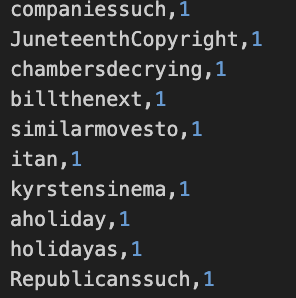
\includegraphics[width=0.4\linewidth]{images/conjoined_words_example.png}
    \caption{Example of conjoined words, over 60 thousand occurences are found within the dataset article contents}
    \label{fig:conjoined_words}
\end{figure}

\begin{figure}[htbp]
    \centering
    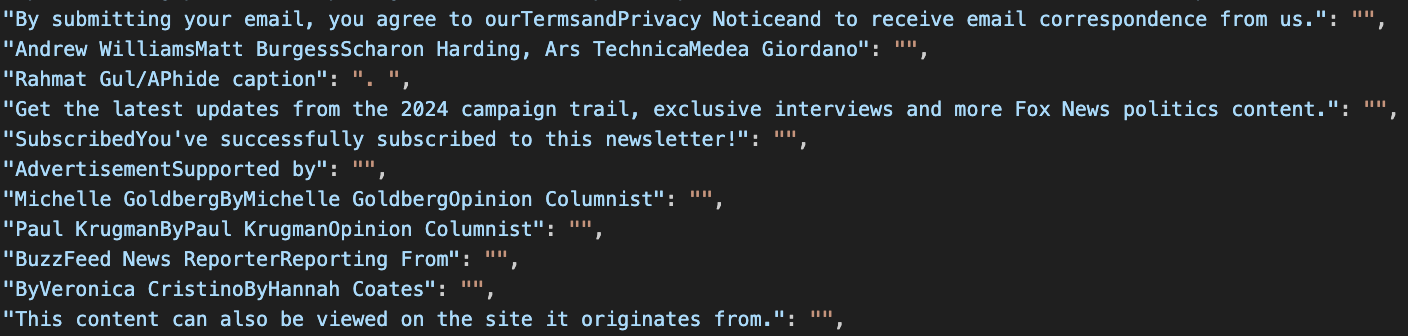
\includegraphics[width=0.67\linewidth]{images/noise_phrases_example.png}
    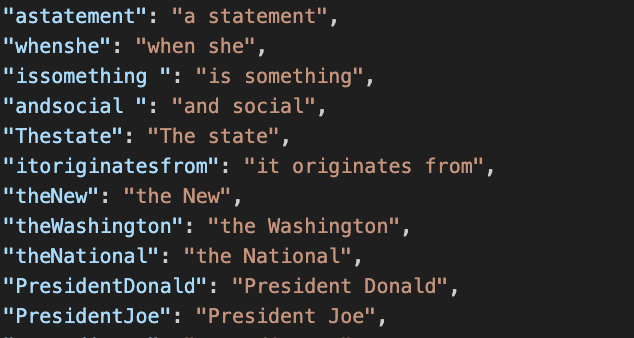
\includegraphics[width=0.3\linewidth]{images/word_fix_example.png}
    \caption{Dictionaries to fix conjoined words and noise phrases}
    \label{fig:dict_fix_examples}
\end{figure}


An additional round of extension is done after the initial scraping by compiling the list of unavailable/unscraped websites and taking a closer look of the problem individually. This round involved searching for missing articles, fixing broken links, visiting the websites manually on the browser, and copy-pasting article contents into a spreadsheet, resulting in additional 226 rows of articles. The final dataset consists of 5496 rows of articles.

\begin{comment}
add total tokens for all contents in the dataset?
add pseudocode for utils and noise fixing?
\end{comment}

\begin{comment}
Explain further on preprocessing scraped text. More details on the preprocessing scripts?
\end{comment}

\section{Analysis}

\begin{figure}[htbp]
    \centering
    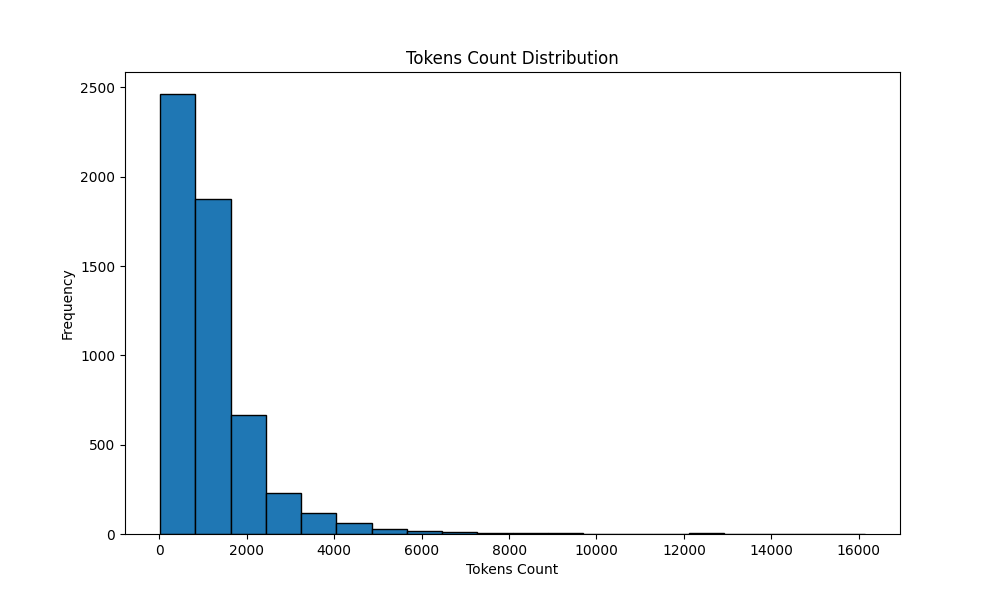
\includegraphics[width=0.9\linewidth]{figures/tokens_count_vx_hist.png}
    \caption{Articles token count distribution}
    \label{fig:tokens_hist}
\end{figure}

\begin{figure}[htbp]
    \centering
    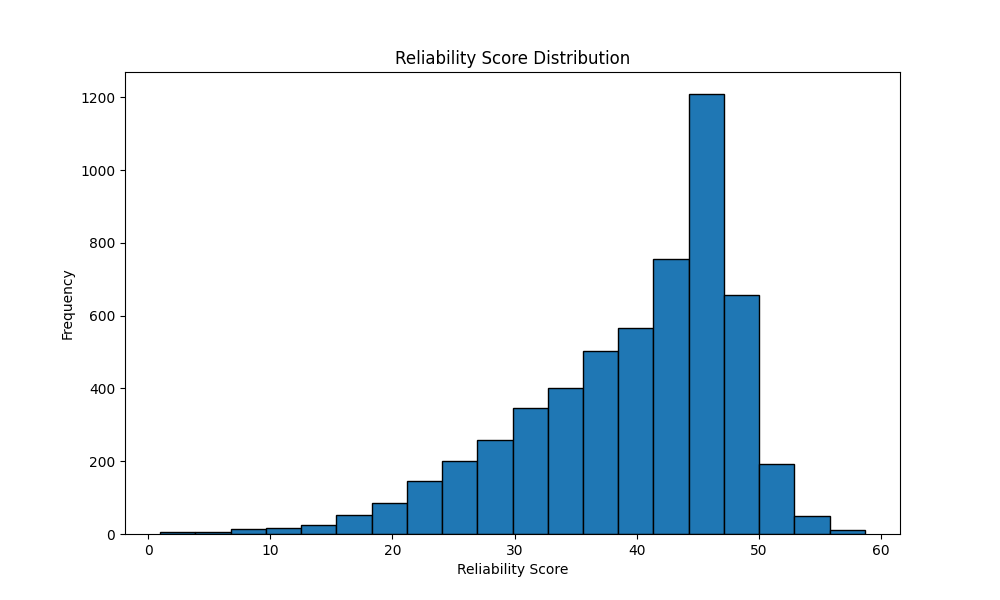
\includegraphics[width=0.9\linewidth]{figures/reliability_score_hist.png}
    \caption{Reliability score distribution}
    \label{fig:reliability_score_hist}
\end{figure}

The article content tokens length ranges between 17 tokens to 16139 tokens, with an average length of 1207.07 and a median value of 908 tokens. Only 9 articles have more than 10000 tokens, while there are 106 of articles with less than 100 tokens. Furthermore, only 1209 articles stay between 512 tokens, which is the limit for BERT input. The articles reliability score ranges from 1.0 to 58.67, the majority have a value between 20 - 50. Not a single articles were rated more than 60 despite the highest score being 64. Visualisations can be seen in both Figure \ref{fig:tokens_hist} and Figure \ref{fig:reliability_score_hist}, as well as Figure \ref{fig:tokens_hist_split}


\begin{figure}[htbp]
    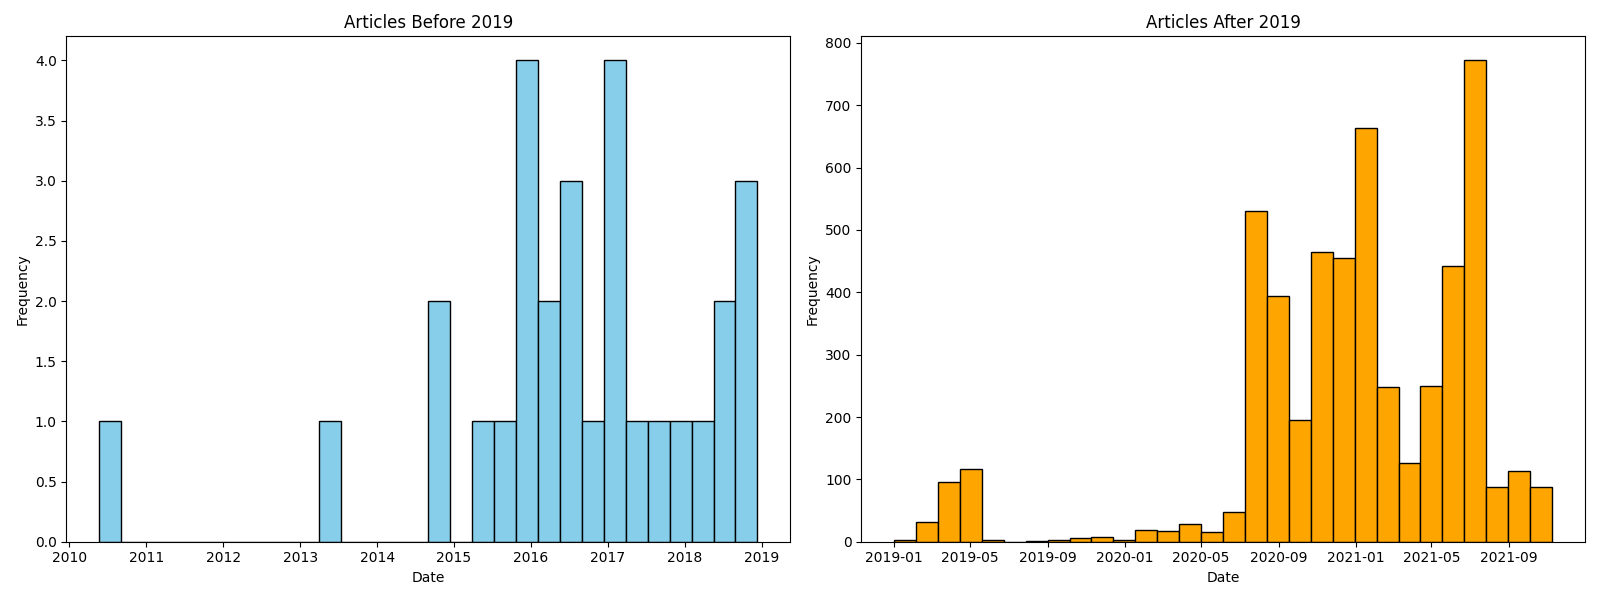
\includegraphics[width=0.9\linewidth]{figures/dates_hist.png}
    \caption{Article dates distribution}
    \label{fig:dates_hist}
\end{figure}

Most articles are written and published within the last 6 years, with only 31 articles, a minuscule percentage, published before 2019, shown in Figure \ref{fig:dates_hist}. From a personal analysis, these 31 articles generally contain similar topics to articles published after 2019 and therefore should not hold consequental difference in behaviour and characteristics.


\begin{figure}[htbp]
    \centering
    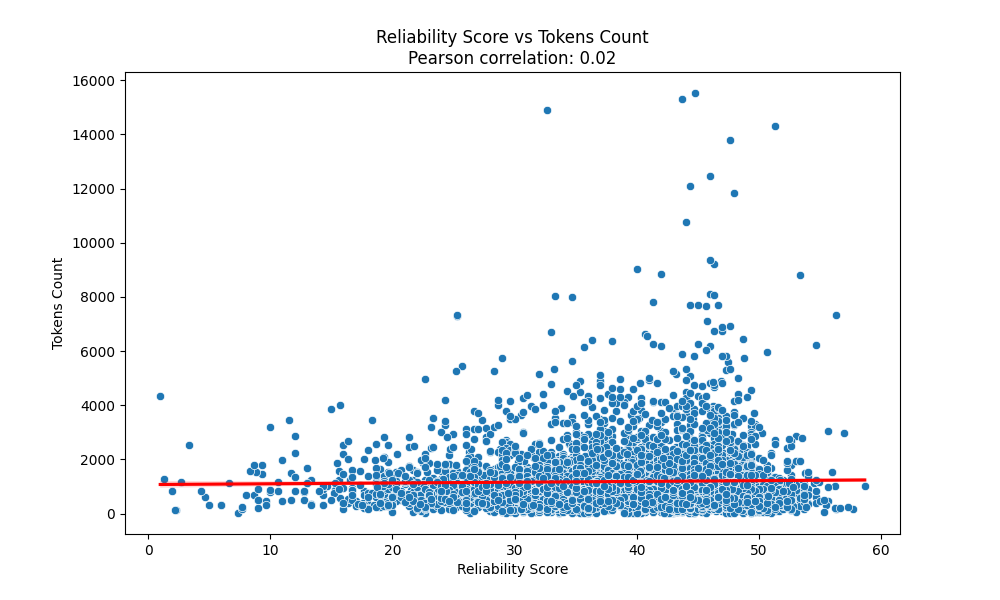
\includegraphics[width=0.9\linewidth]{figures/correlation_tokens_reliability_score.png}
    \caption{Pearson correlation between token count and reliability score}
    \label{fig:pearson_correlation}
\end{figure}


\begin{figure}[htbp]
    \centering
    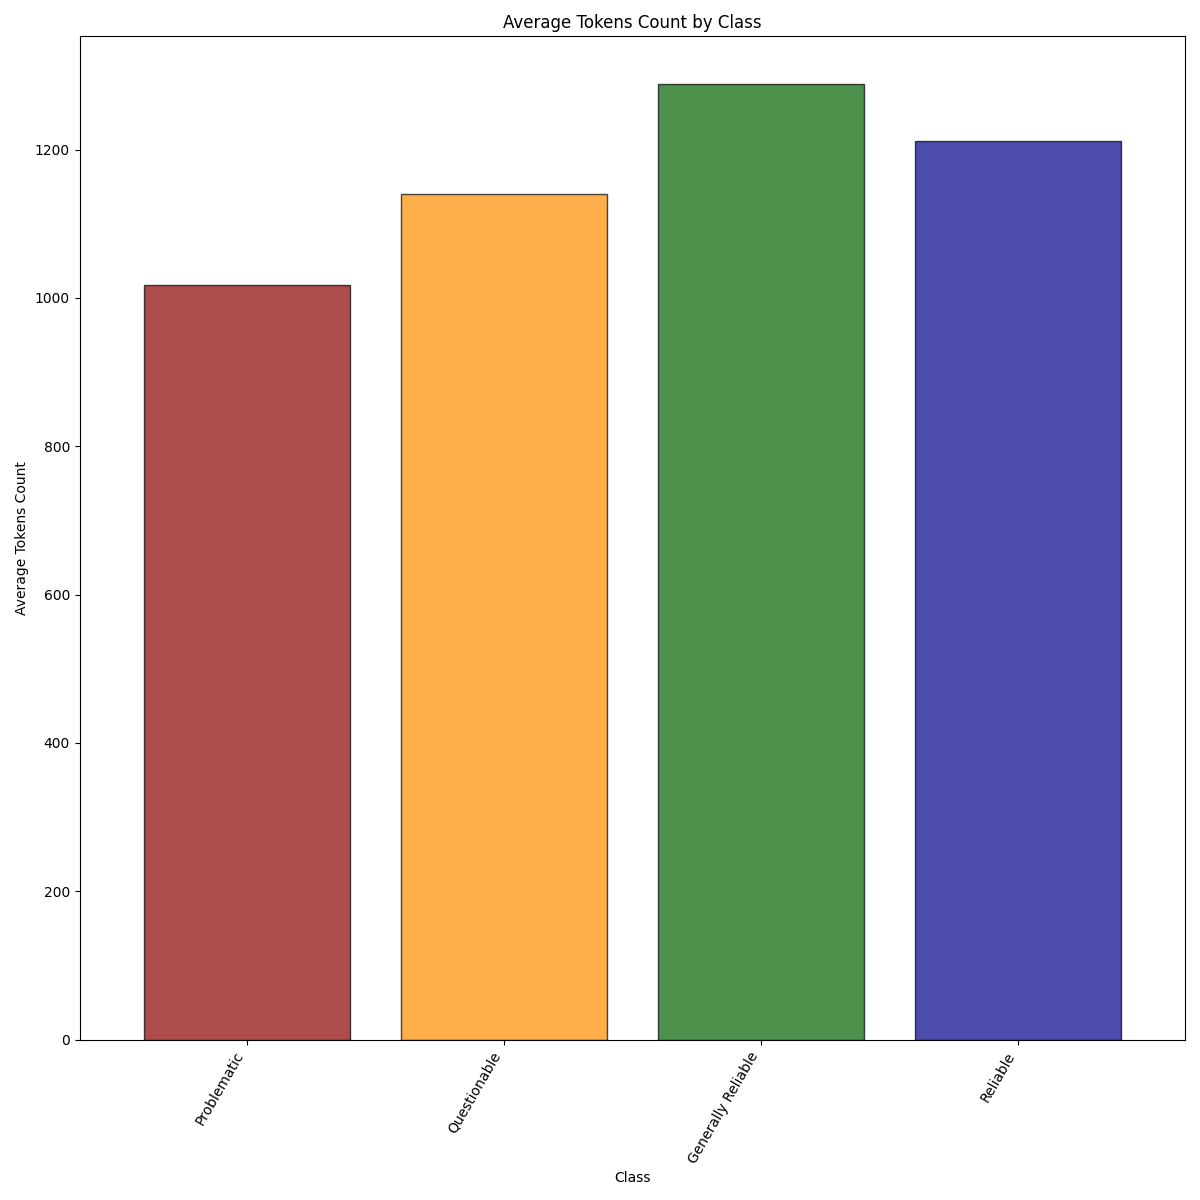
\includegraphics[width=0.8\linewidth]{figures/tokens_count_vx_per_class_hist.png}
    \caption{Average tokens count per class}
    \label{fig:avg_tokens_count_per_class}
\end{figure}

Figure \ref{fig:avg_tokens_count_per_class} shows that all classes seem to have similar token count, close to the overall average. Class 'Problematic' and 'Questionable', being the two most biased classes, seem to have lower average token count than the two other classes. However, further analysis (Figure \ref{fig:pearson_correlation}) shows that there is virtually no linear relationship between token count and reliability score, with a Pearson correlation coefficient is 0.02. This proves that the length of an article has no significant impact on its reliability score. In other words, longer articles are not necessarily more or less reliable than shorter ones based on the provided data.

\begin{comment}
relationship between words and reliability score?
\end{comment}


%%% Local Variables: 
%%% mode: latex
%%% TeX-master: "thesis"
%%% End: 